% !TEX root = ../Dokumentation.tex
\subsection{Gesamtübersicht}

\begin{figure}[h!]%Position festigen
\centering
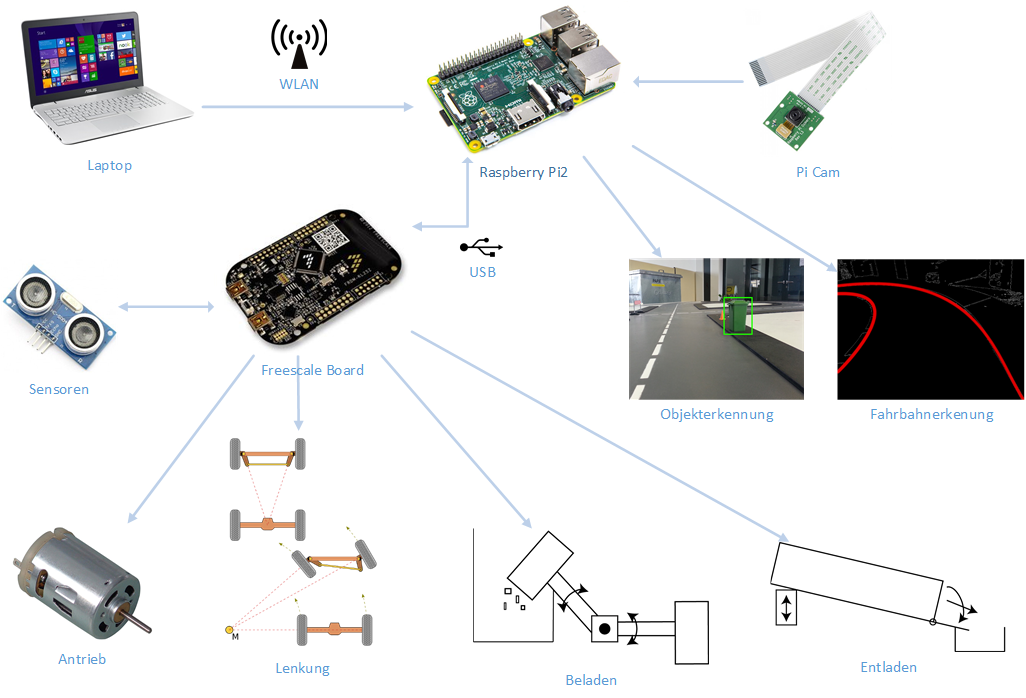
\includegraphics[width=0.9\textwidth]{03_Loesungskonzept/pictures/uebersichtszeichnung.png}
\caption{Übersichtszeichnung}
\label{fig:Java}
\end{figure}

\subsubsection{Zusammenspiel}
\textbf{Funktionsbeschrieb}
\textbf{Komponentenbeschrieb}
\textbf{Begründung}
Wenn benötigt
\textbf{Berechnungen}
\textbf{Testergebnisse}

\subsubsection{Schnittstellen}
\textbf{Funktionsbeschrieb}
\textbf{Komponentenbeschrieb}
\textbf{Begründung}
Wenn benötigt
\textbf{Berechnungen}
\textbf{Testergebnisse}